\chapter{Wstęp}

\section{Znaczenie losowości w systemach brzegowych}

\noindent Rosnąca złożoność systemów informatycznych wymusza na inżynierach 
wdrażanie nowych rozwiązań technicznych. W odpowiedzi na znaczne 
uzależnienie systemów informatycznych od usług chmurowych powstała dziedzina 
przetwarzania brzegowego (ang. \textit{edge computing}). Zakłada ona ograniczenie 
interakcji z chmurą poprzez rozwój dedykowanych systemów brzegowych. Podejście 
to opiera się na przetwarzaniu danych oraz podejmowaniu decyzji przez system 
bezpośrednio w miejscu, w którym te dane są generowane.

Podejście to ogranicza zależność od systemów chmurowych, jednak wprowadza nowe 
zagrożenia charakterystyczne dla tej klasy systemów. Wiele rozwiązań opartych 
jest na układach scalonych przeznaczonych do konkretnych zastosowań (ang. \textit{ASIC} --
 \textit{Application-Specific Integrated Circuit}). Ich główną zaletą jest 
 znaczna adaptowalność do zadań, które mają wykonywać. Jest to jednak 
 opłacone dużą złożonością rozwijanego systemu, co otwiera go na nowe podatności. 
 Jedną ze szczególnych klas zagrożeń, wynikających ze złożonego procesu rozwoju, są trojany 
 sprzętowe wprowadzane przez atakującego na etapach projektowania i produkcji 
 układów scalonych.

Ze względu na powagę tego zagrożenia przyjęto, że jedną z metod przeciwdziałania 
jest promowanie układów scalonych rozwijanych w sposób transparentny i 
weryfikowalny. Organizacje takie jak OSHWA (ang. \textit{Open-Source Hardware Association}) 
i projekty takie jak RISC-V stanowią fundament ruchu wspierającego transparentny 
rozwój otwartoźródłowych rozwiązań technicznych.

OSHWA oraz architektura zestawu instrukcji RISC-V stanowią odpowiedź na kryzys 
zaufania do zamkniętych i komercyjnych architektur. Znajdują się 
we wspólnym ekosystemie otwartoźródłowych technologii, choć pełnią różne 
funkcje. Architektura RISC-V jest jedynie standardem technicznym, który 
umożliwia rozwój układów scalonych. Z kolei OSHWA jest organem nadzorującym 
rozpowszechnianie konkretnych, gotowych rozwiązań. Połączenie projektu i ogranizacji 
poskutkowało powstaniem szerokiego wachlarza transparentnych, otwartoźródłowych 
i bezpiecznych projektów układów scalonych.

Generatory liczb losowych stanowią istotną część algorytmów 
współczesnej kryptografii~\cite{2016Sreekumar-Ramesh}. Liczby losowe 
wykorzystywane są w kryptografii na różnych etapach i w wielu 
różnych celach.

Generowanie par kluczy kryptograficznych algorytmem RSA zapewnia bezpieczeństwo 
komunikacji przy założeniu wysokiej złożoności obliczeniowej faktoryzacji iloczynu 
dwóch losowych liczb pierwszych~\cite{Handbook-of-Applied-Cryptography}. 
Dopiero gdy dane liczby pierwsze spełniają kryteria oceny losowości, możemy 
stwierdzić, że para kluczy będzie bezpieczna. Oznacza to, że próba 
faktoryzacji będzie na tyle wymagająca sprzętowo i czasowo, aby uczynić ją 
nieopłacalną dla atakującego.

Tworzenie podpisów cyfrowych nie byłoby możliwe bez odpowiednich źródeł 
losowości. Kryptografia krzywych eliptycznych, stosowana przy podpisywaniu 
plików binarnych, zawiera element losowy w postaci jednorazowej wartości nonce. 
Sytuacja, w której nonce nie spełnia miar losowości, naraża na niebezpieczeństwo 
cały klucz prywatny producenta. Gdy kilka kolejnych bitów losowych wartości nonce 
(używanych przy każdej generacji sygnatury) jest znanych dla pewnej liczby 
sygnatur cyfrowych, możliwe jest odzyskanie klucza 
prywatnego~\cite{ch1-the-insecurity-of-ECDSA}.

W różnych trybach pracy szyfrów blokowych, takich jak AES, wprowadzane są 
dodatkowe wartości losowe, takie jak wektor inicjalizacyjny (IV) czy nonce. Powtarzająca się 
wartość nonce w trybie AES-CTR naraża na niebezpieczeństwo całą szyfrowaną wiadomość. 
Przechwycenie dwóch różnych szyfrogramów wygnerowanych z tym samym nonce 
umożliwia wydobycie tekstu jawnego~\cite{NIST-SP-800-38A}.

Przesłanki te stanowią motywację do podjęcia badań nad oceną dostępnych 
generatorów losowości.

Projekt „The NEORV32 RISC-V Processor” jest jedną z realizacji idei OSHWA i 
RISC-V. Jest to otwartoźródłowa, modyfikowalna platforma sprzętowa napisana w 
języku opisu sprzętu VHDL. Rozwiązanie to jest dedykowane inżynierom rozwijającym 
systemy brzegowe w oparciu o układy FPGA.

W strukturze procesora NEORV32 RISC-V zintegrowano moduł generatora entropii 
neoTRNG, który stanowi główny przedmiot badań prowadzonych w ramach niniejszej 
pracy magisterskiej. Podjęcie tematyki weryfikacji oraz analizy zastosowanego 
generatora pozwala na realny wkład w rozwój bezpieczeństwa 
technologii otwartoźródłowych.




\section{Cel pracy}

\noindent Celem niniejszej pracy magisterskiej jest adaptacja oraz 
implementacja otwartoźródłowego generatora losowości neoTRNG, bazującego na 
oscylatorach pierścieniowych. Badany moduł będzie implementowany jako układ 
cyfrowy realizowany na płycie deweloperskiej wyposażonej w układ FPGA. Badania 
zostaną przeprowadzone za pomocą dedykowanego środowiska testowego. 

Kryteria oceny generatora obejmować będą: zestaw testów statystycznych 
zdefiniowanych w publikacji NIST SP 800-22~\cite{NIST-SP-800-22}, 
zestaw testów do oceny entropii opisany w publikacji 
NIST SP 800-90B~\cite{NIST-SP-800-90B} oraz program do oceny 
generatorów pseudolosowych ENT~\cite{fourmilab-ENT}. Wraz z wynikami testów 
zestawione zostaną informacje o zajętości zasobów sprzętowych 
i przepustowości poszczególnych implementacji. Badane moduły będą 
stanowić modyfikacje bazowego rozwiązania neoTRNG przedstawionego 
w repozytorium~\cite{neoTRNG}. Modyfikacje obejmą aspekty takie jak: 
liczba zastosowanych oscylatorów, zastosowanie korekcji źródła 
(np. korektor Von Neumanna), metody przetwarzania końcowego 
(ang. \textit{post-processing}) oraz fizyczne rozmieszczenie elementów w strukturze FPGA.






% \section{Charakterystyka literatury}

% \noindent Badania zostaną przeprowadzone na podstawie rekomendacji branżowych 
% dotyczących projektowania źródeł entropii oraz publikacji naukowych związanych 
% z analizowaną tematyką.

\section{Układ pracy}

\noindent Struktura pracy obejmuje pięć rozdziałów oraz dodatkową sekcję załączników. 

Rozdział pierwszy przedstawia motywację podjęcia badań w obszarze generatorów 
losowości oraz określa założenia i cele pracy. 

Rozdział drugi koncentruje się na podstawach teoretycznych. Omówiono w nim 
definicje związane z tematyką pracy, dostępne ekstraktory entropii oraz metody 
oceny losowości.

Rozdział trzeci omawia architekturę badanego modułu neoTRNG oraz przedstawia 
różne modyfikacje badanego generatora wraz z analizą ich zajętości sprzętowej.  

Rozdział czwarty poświęcono badaniom eksperymentalnym. Zbadane zostaną: 
\begin{itemize}
    \item wpływ metod post-processing'u na losowość, 
    \item wpływ skalowania liczby oscylatorów pierścieniowych oraz liczby 
    inwerterów na losowość, 
    \item wpływ zastosowania ekstraktorów AES-CTR i Toeplitza na losowość, 
    \item wpływ rozmieszczenia komórek entropii w układzie FPGA na losowość. 
\end{itemize}

Wraz z wynikami testów losowości dołączona zostanie informacja o przepustowości 
każdej z implementacji.

Rozdział piąty kończy pracę i podsumowuje najważniejsze wnioski wynikające z 
przeprowadzonych badań.

Załącznik A zawiera instrukcję planowania rozmieszczenia elementów 
(ang. \textit{floorplanning}), wykonanego w ramach analizy rozmieszczenia 
komórek entropii.

Załącznik B zawiera instrukcję przedstawiającą metodę akwizycji oraz przetworzenia 
danych testowych.

\chapter{Teoretyczne aspekty projektowania sprzętowych generatorów liczb losowych}

% Rozdział teoretyczny --- przegląd literatury naświetlający stan wiedzy na dany temat. 

% Przegląd literatury naświetlający stan wiedzy na dany temat obejmuje rozdziały pisane na podstawie
% literatury, której wykaz zamieszczany jest w części pracy pt.~\emph{Literatura} (lub inaczej \emph{Bibliografia},
% \emph{Piśmiennictwo}). W tekście pracy muszą wystąpić odwołania do wszystkich pozycji zamieszczonych w
% wykazie literatury. \textbf{Nie należy odnośników do literatury umieszczać w stopce strony.} Student jest
% bezwzględnie zobowiązany do wskazywania źródeł pochodzenia informacji przedstawianych w pracy,
% dotyczy to również rysunków, tabel, fragmentów kodu źródłowego programów itd. Należy także podać
% adresy stron internetowych w przypadku źródeł pochodzących z Internetu.

\noindent Niniejszy rozdział przedstawia teoretyczne podstawy projektowania 
sprzętowych generatorów liczb losowych. Omówiono w nim klasyfikację architektur 
generatorów oraz zjawiska fizyczne wykorzystywane do pozyskiwania entropii w 
układach programowalnych FPGA. Ponadto wyjaśniono metody obróbki sygnałów 
losowych, a także standardy statystyczne stosowane do walidacji jakości 
generowanych danych.

\section{Źródła losowości}

\noindent Generatory liczb losowych można podzielić na kategorie w zależności 
od mechanizmu powstawania losowości. Dwie główne klasy generatorów stanowią 
generatory liczb prawdziwie losowych (ang. \textit{TRNG} -- \textit{True Random Number Generator}) 
oraz generatory liczb pseudolosowych (ang. \textit{PRNG} -- \textit{Pseudorandom Number Generator}). 

Spośród generatorów liczb prawdziwie losowych można wyróżnić podklasę 
kwantowych generatorów liczb prawdziwie losowych (ang. \textit{QRNG} -- \textit{Quantum Random Number 
Generator})~\cite{2025QRNG-zeshan}.

Podklasą generatorów pseudolosowych są generatory pseudolosowe kryptograficznie 
bezpieczne (ang. \textit{CSPRNG} -- \textit{Cryptographically Secure Pseudorandom Number Generator}). 

Kryterium podziału generatorów na TRNG i PRNG jest źródło pochodzenia losowości. 


\subsection{TRNG}

\noindent Generatory liczb prawdziwie losowych opierają generowanie liczb na 
digitalizacji niedeterministycznych zjawisk fizycznych. 
Przykładowymi źródłami szumów analogowych są: 
szum napięcia zasilania, fluktuacje temperatury elementów pasywnych, 
niestabilności fazowe w układach cyfrowych (oscylatory pierścieniowe) lub 
bardziej nietypowe zjawiska, takie jak procesy kwantowe w układach optycznych. 

\begin{figure}[H]
    \centering
    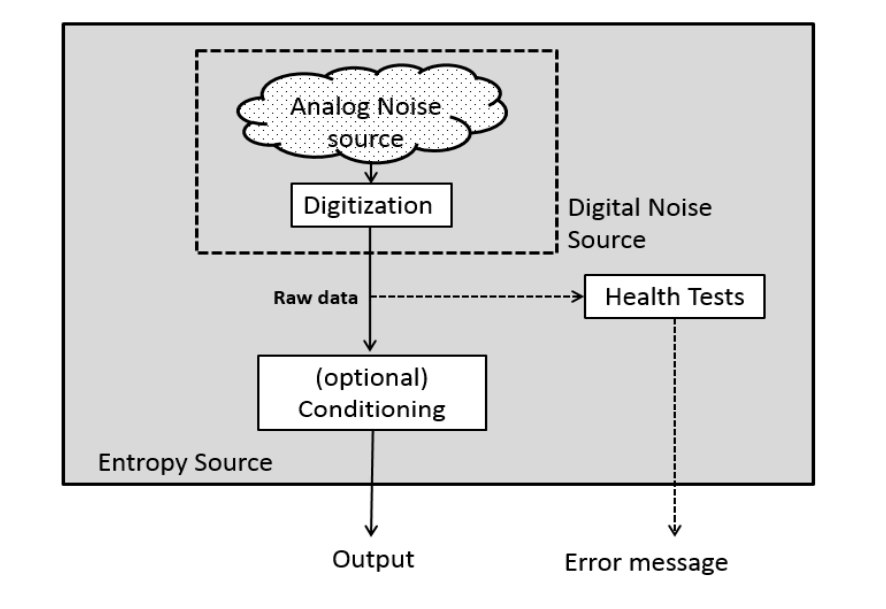
\includegraphics[width=0.75\textwidth]{figures/ch2/nist_source_schematic.png}
    \caption{Model źródła entropii.~\cite{NIST-SP-800-90B}}
    \label{fig:ch2_model_zrodla_entropii_nist}
\end{figure}

Wiodącą publikacją w dziedzinie projektowania generatorów liczb prawdziwie 
losowych jest zbiór rekomendacji projektowych \textit{NIST SP 800-90B}. 
Publikacja ta opisuje ogólny model źródła losowości złożony z czterech 
części składowych~\cite{NIST-SP-800-90B}:

\begin{itemize}
    \item źródło szumu analogowego -- entropia zbierana z niedeterministycznego 
    procesu fizycznego,
    \item digitalizacja -- próbkowanie oraz kwantyzacja sygnału analogowego 
    poprzez np. przetwornik analogowo-cyfrowy,
    \item przetwarzanie końcowe -- metody postprocessing'u w celu zwiększenia 
    jakości wygenerowanej entropii, 
    \item testy zdrowia -- moduły monitorujące pracę źródła, wykrywające awarie i 
    próby manipulacji.
\end{itemize}

Mimo wielu zalet generatory liczb prawdziwie losowych nie są całkowicie 
odporne na ataki. Możliwą formą ataku jest zakłócenie źródła szumu analogowego, 
na przykład poprzez rozgrzanie termistora próbkującego fluktuacje temperatury.

\subsection{PRNG}

\noindent Generatory liczb pseudolosowych charakteryzują się generowaniem sygnału 
pozornie losowego. Wynika to z mechanizmów wewnątrz takiego generatora. 
\enquote{Generowanie liczb pseudolosowych polega na tworzeniu długich sekwencji 
bitów, zaczynając od małej, najlepiej prawdziwie losowej wartości początkowej 
zwanej ziarnem}~\cite{2023anstasios-panagiotis-georgis-yannis}. Główną wadą 
takich generatorów jest przewidywalność całego ciągu losowego po poznaniu 
wykorzystanego ziarna. 

Bazują one na podstawowych operacjach algebraicznych, generując kolejne 
wartości na podstawie wyników powtarzających się obliczeń. Z tego względu 
klasyczne algorytmy PRNG (LCG, Mersenne Twister) nie są uważane za generatory 
bezpieczne kryptograficznie. Są one podatne na analizę sekwencji ciągu, co 
umożliwia przewidzenie kolejnych wygenerowanych 
wartości~\cite{2024-predicting-prngs}.

Ze względu na ich prostotę znajdują one zastosowanie w systemach niekrytycznych. 
Są stosowane przy generowaniu proceduralnym bądź w symulacjach naukowych.

\subsection{CSPRNG}

\noindent Kryptograficznie bezpieczne generatory liczb pseudolosowych działają 
w sposób analityczny jak generatory PRNG, z jedną szczególną różnicą: 
wykorzystują nieodwracalne funkcje kryptograficzne. Tego typu generatory 
muszą spełniać dwa wymagania: test następnego bitu (ang. \textit{next-bit test}) oraz odporność na kompromitację 
stanu~\cite{2023Analisis-of-CSPRNG}. 

Oznacza to, że poprzez znajomość ciągu $N$ bitów losowych atakujący nie jest 
w stanie przewidzieć bitu $N+1$ z prawdopodobieństwem większym niż 50\% oraz, 
znając część lub całość stanu generatora, nie jest w stanie odtworzyć 
poprzednich wygenerowanych wartości~\cite{2023Analisis-of-CSPRNG}.

\subsection{QRNG}

\noindent Kwantowe generatory liczb losowych stanowią szczególny przypadek 
generatora prawdziwie losowego. Zamiast pobierać entropię ze zjawisk fizyki 
klasycznej, wykorzystują zjawiska mechaniki kwantowej. 

Ich główną przewagą jest probabilistyczna natura zjawisk kwantowych. Zjawiska 
fizyki klasycznej, takie jak zmiany temperatury, można zamodelować za pomocą cząstkowych 
równań różniczkowych, co może dać niepożądany wgląd do wnętrza mechanizmu 
generującego losowość. W przypadku zjawisk kwantowych modele takie nie 
istnieją -- obserwowany układ kwantowy zawsze będzie działał z określonym 
rozkładem prawdopodobieństwa~\cite{Quantum-physics-peter-kok}. 

Wadą kwantowych generatorów jest ich cena. Zazwyczaj rozwiązania kwantowe są 
znacznie droższe niż generatory klasyczne.

\subsection{Zasada działania Quantis USB 4M}

\noindent Komercyjnie dostępny jest kwantowy generator Quantis-USB-4M firmy IDQ. 
Urządzenie to dostępne w obudowie z interfejsem USB 2.0.

\begin{figure}[H]
    \centering
    
\includegraphics[width=0.4\textwidth]{figures/ch2/Quantis-QRNG-USB.png}
    \caption{Quantis USB 4M.~\cite{quatis-brouchure}}
    \label{fig:ch2_qunatis-usb}
\end{figure}


\begin{table}[htbp]
\centering
\caption{Specyfikacja ogólna urządzenia Quantis-USB-4M~\cite{quatis-brouchure}}
\label{tab:quantis_usb_specs}
\begin{tabular}{p{5.5cm}l}
\toprule
\textbf{Parametr} & \textbf{Specyfikacja} \\
\midrule
Losowa prędkość bitowa* & 4 Mbit/s $\pm$ 10\% \\
Udział szumu termicznego & $< 1\%$ \\
Temperatura przechowywania & od -25 do +85°C \\
Wymiary & 61 mm $\times$ 31 mm $\times$ 114 mm \\
Specyfikacja USB & 2.0 \\
Wymagania & Komputer PC z wolnym złączem USB \\
Zasilanie & Przez port USB \\
\bottomrule
\end{tabular}
\par\vspace{2mm}    
\begin{minipage}{0.5\textwidth} 
\small
* Przepustowość (bitrate) przed ekstrakcją losowości
\end{minipage}
\end{table}

Według specyfikacji producenta (Tab.~\ref{tab:quantis_usb_specs}) udział szumu 
termicznego w generowanych bitach losowych wynosi mniej niż 1\%. Oznacza to, 
że generator wytwarza losowość niemal wyłącznie ze zjawisk mechaniki kwantowej.


\begin{figure}[H]
    \centering
    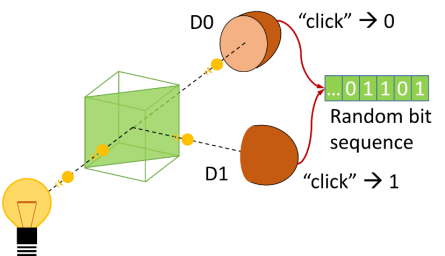
\includegraphics[width=0.6\textwidth]{figures/ch2/319_QNRG.png}
    \caption{Model układu optycznego.~\cite{Quantum-randomness-generator-optical-circ}}
    \label{fig:ch2-model-ukladu-kwantowego}
\end{figure}

Układ optyczny znajdujący się wewnątrz Quantis USB 4M składa się z trzech elementów:

\begin{itemize}
    \item źródła fotonów -- laser o niskiej mocy generujący wiązkę fotonów,
    \item dzielnika wiązki -- pryzmat wykonany z materiałów, które częściowo 
    przepuszczają fotony,
    \item dwóch detektorów fotonów.
\end{itemize}

Generowana losowość jest związana z częściową przepuszczalnością dzielnika 
wiązki. W przypadku idealnym 50\% fotonów zostaje odbitych, a 50\% zostaje 
przepuszczonych. Oznacza to, że prawdopodobieństwo detekcji fotonu w każdym 
z detektorów jest rozłożone równo po 50\%. W ten sposób generator kwantowy 
wytwarza ciąg bitów niedeterministycznych z jednostajnym rozkładem bitu '1' i '0'.

Jednak w rzeczywistości dzielnik wiązki nie jest elementem idealnym. Oznacza 
to, że prawdopodobieństwo wystąpienia bitu '1' lub '0' nie będzie równe idealnie 50\%. 

\section{RO jako źródło losowości w FPGA}

\noindent Generowanie losowości przy użyciu oscylatorów pierścieniowych bazuje 
na zjawiskach fizycznych związanych z propagacją sygnałów wewnątrz 
struktury krzemowej układu FPGA. Oscylator pierścieniowy 
(ang. \textit{RO} -- \textit{Ring Oscillator}) jest asynchronicznym układem cyfrowym złożonym z 
pętli o nieparzystej liczbie inwerterów. 

\begin{figure}[H]
    \centering
    \includesvg[width=\textwidth]{figures/ch2/schematic.svg}
    \caption{Przykład prostego oscylatora pierścieniowego.}
    \label{fig:ch2_oscylator_3xNOT}
\end{figure}

Tak skonstruowany układ logiczny doprowadzi do powstania stanu nieustalonego 
wewnątrz układu. Inwertery ułożone w pętli będą kolejno generować sygnał 
wejściowy dla następnego inwertera w kolejności. Oznacza to, że w układzie 
powstanie sygnał oscylujący z okresem wynikającym z czasu propagacji sygnału 
w krzemie oraz liczby zastosowanych inwerterów. Należy zwrócić uwagę, że ma 
to zastosowanie wyłącznie dla nieparzystej liczby inwerterów. W przypadku liczby 
parzystej sygnał się ustali, a próbkowane wyjście będzie zwracać wartość stałą.

\begin{figure}[H]
    \centering
    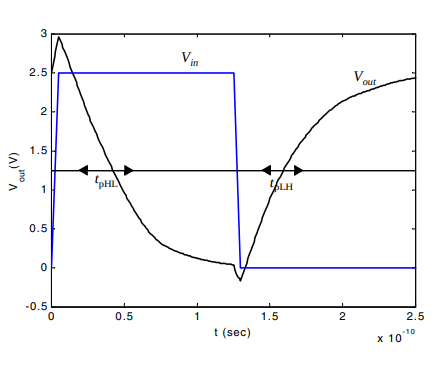
\includegraphics[width=0.6\textwidth]{figures/ch2/inverter.png}
    \caption{Propagacja sygnału wewnątrz inwertera CMOS -- symulacja.~\cite{Digital-integraged-circuits-A-design-perspective}}
    \label{fig:ch2_inverter_propagation}
\end{figure}

Na zamieszczonym rysunku (Fig.~\ref{fig:ch2_inverter_propagation}) przedstawiono 
przebiegi sygnału $V_{in}$ oraz $V_{out}$ dla symulacji inwertera wykonanego 
w technologii $0.25 \mu m$. Widoczne jest opóźnienie w propagacji sygnału 
wyjściowego dla skokowej zmiany sygnału wejściowego. Od momentu przełączenia 
$V_{in}$ do ustalenia sygnału $V_{out}$ na poziomie 2.5 V mija 
około $100~\text{ps}$.

W rzeczywistości każdy inwerter będzie odrobinę różnić się od reszty ze 
względu na niedoskonałe metody produkcyjne. Co za tym idzie, sygnał wyjściowy 
z RO będzie zmieniał się w jeszcze bardziej nieprzewidywalny sposób. Idąc 
dalej, pozwala to na stworzenie układu składającego się z wielu RO o różnej liczbie inwerterów, 
gdzie kombinacja ich wyjść wygeneruje porządaną losowość. Umożliwia to 
opracowanie generatora liczb prawdziwie losowych ze względu na analogową 
naturę zjawisk zachodzących wewnątrz układu RO.

\section{Ekstraktory losowości}

\noindent Sygnał pozyskiwany bezpośrednio ze źródła analogowego charakteryzuje się 
niejednostajnym rozkładem zer i jedynek oraz występowaniem korelacji. Aby poprawić 
losowość, sugerowaną praktyką jest odpowiednia korekcja ciągu bitów. 

\subsection{Ekstraktor von Neumanna}

\noindent Ekstraktor von Neumanna jest nieskomplikowanym układem cyfrowym. 
Jego zadaniem jest zapewnienie jednostajnego rozkładu generowanych liczb losowych. 
Zasada działania tego ekstraktora opiera się na pobraniu dwóch próbek sygnału ze 
źródła oraz sprawdzeniu zestawu trzech instrukcji:

\begin{itemize}
    \item pobrano próbki $(0;0)$ lub $(1;1)$ $\rightarrow$ próbki zostają odrzucone,
    \item pobrano próbki $(1;0)$ $\rightarrow$ generowany jest bit $1$,
    \item pobrano próbki $(0;1)$ $\rightarrow$ generowany jest bit $0$.
\end{itemize}

Ekstraktor zapewnia jednostajny rozkład prawdopodobieństwa wystąpienia 
każdego z bitów, ale znacznie ogranicza przepustowość generatora. Jednocześnie 
nie pozbywa się on korelacji z generowanego sygnału. 

\subsection{Wielomian CRC}

\noindent Cykliczna kontrola nadmiarowa (ang. \textit{CRC} -- \textit{Cyclic Redundancy Check}) jest 
pierwotnie stosowana w celu zapewnienia integralności przesyłanych danych w 
interfejsach komunikacyjnych~\cite{ucgosu-CRC}. Znajduje jednak również 
zastosowanie w korekcji źródła losowości. 

Zaimplementowana jest w postaci liniowego rejestru przesuwającego ze 
sprzężeniem zwrotnym (LFSR). Posiada właściwości rozpraszające, co oznacza, że każdy nowy 
bit ma wpływ jednocześnie na wszystkie bity wyjściowe. W ten sposób eliminuje 
korelacje między wyjściowymi bitami.


\subsection{Ekstraktor Toeplitza}

\noindent Ekstraktor oparty na macierzach Toeplitza należy do grupy silnych 
ekstraktorów losowości (ang. \emph{strong extractors}). Ekstrakcja polega na 
pomnożeniu wektora surowych bitów wejściowych $X$ o długości $n$ przez macierz 
Toeplitza $M$ o wymiarach $m \times n$ (gdzie $m < n$):
\begin{equation}
    Y = M \cdot X
\end{equation}
Macierz Toeplitza ma tę właściwość, że każdy jej ukośny rząd ma stałą wartość, 
co pozwala na jej jednoznaczne zdefiniowanie za pomocą jedynie $n + m - 1$ 
bitów ziarna.

\subsection{Szyfr strumieniowy AES-CTR}

\noindent Szyfr blokowy AES działający w trybie licznika jest jednym z zalecanych 
systemów generowania liczb losowych. Konfiguracja AES-CTR polega na ciągłym generowaniu 
losowego szyfrogramu na podstawie wstępnej wartości ziarna pobranej ze źródła 
losowości. 

Na początku pracy AES-CTR pobierane są losowe wartości klucza oraz nonce. Tekst jawny jest 
połączeniem nonce oraz wartości z licznika. Taka konfiguracja pozwala 
wygenerować spore ilości danych losowych dla kolejnym wartości z licznika 
przy niewielkim wykorzystaniu źródła losowości. 

Wadą tego podejścia jest cykliczna konieczność odświeżania ziarna wykorzystanego 
na początku procesu.  

\section{Metody oceny losowości}

\noindent Ocena właściwości statystycznych generatora liczb losowych złożona jest z 
zestawu miar i testów. W ramach badań wykorzystuje się publicznie dostępne 
programy do oceny generowanych ciągów losowych. 


\subsection{Program ENT}

\noindent \enquote{Program ENT przeprowadza różne testy 
na sekwencjach bajtów zapisanych w plikach i raportuje wyniki tych testów. Program jest 
przydatny do oceny generatorów liczb pseudolosowych w zastosowaniach szyfrowania i 
próbkowania statystycznego, algorytmach kompresji i innych zastosowaniach, w których 
istotna jest gęstość informacji w pliku}~\cite{fourmilab-ENT}.

\begin{figure}[H]
    \centering
    \begin{minted}[linenos, breaklines, breakanywhere]{bash}
Entropy = 7.168778 bits per byte.

Optimum compression would reduce the size
of this 104857600 byte file by 10 percent.

Chi square distribution for 104857600 samples is 131655940.14, and randomly
would exceed this value less than 0.01 percent of the times.

Arithmetic mean value of data bytes is 127.4529 (127.5 = random).
Monte Carlo value for Pi is 3.458389109 (error 10.08 percent).
Serial correlation coefficient is 0.000098 (totally uncorrelated = 0.0).
    \end{minted}
    \caption{Przykładowy wynik pakietu ENT.}
    \label{fig:ch2_wyniki_ent}
\end{figure}


\subsection{NIST SP 800-22 -- Zestaw testów statystycznych dla generatorów liczb 
losowych i pseudolosowych do zastosowań kryptograficznych}

\noindent Zestaw testowy NIST SP 800-22 jest standardowym kryterium oceny 
generatorów liczb losowych. Składa się z piętnastu testów odpowiedzialnych za 
sprawdzenie różnych aspektów wygenerowanego ciągu bitów.

\begin{table}[htbp]
\centering
\caption{Opis 15 testów statystycznych pakietu NIST SP 800-22 Rev. 1a~\cite{NIST-SP-800-22}}
\label{tab:nist_tests}
\vspace{2mm}
\footnotesize % Zmniejszenie czcionki, aby tabela zmieściła się na jednej stronie
\begin{tabularx}{\textwidth}{lX p{9.5cm}}
\toprule
\textbf{Lp.} & \textbf{Nazwa testu (ang.)} & \textbf{Krótki opis i cel testu} \\
\midrule
1 & Frequency (Monobit) Test & Badanie proporcji jedynek do zer w całym ciągu binarnym. Sprawdza, czy ich liczba jest w przybliżeniu równa. \\
2 & Frequency Test within a Block & Badanie proporcji jedynek do zer wewnątrz mniejszych, określonych bloków bitów wyciętych z ciągu. \\
3 & Runs Test & Badanie całkowitej liczby serii (nieprzerwanych ciągów samych jedynek lub samych zer) o różnych długościach. \\
4 & Test for the Longest Run of Ones in a Block & Test bada długość najdłuższej serii jedynek w blokach $M$-bitowych i sprawdza, czy jest ona zgodna z wartością oczekiwaną dla ciągu losowego. \\
5 & Binary Matrix Rank Test & Test wyznacza rząd rozłącznych podmacierzy binarnych, aby sprawdzić liniową zależność między podciągami o stałej długości. \\
6 & Discrete Fourier Transform (Spectral) Test & Test analizuje wysokość szczytów transformaty Fouriera (DFT) ciągu, aby wykryć bliskie, powtarzające się wzorce okresowe przeczące losowości ciągu. \\
7 & Non-overlapping Template Matching Test & Zliczanie wystąpień określonych, nienakładających się wzorców bitowych (szablonów) w celu wykrycia anomalii struktur. \\
8 & Overlapping Template Matching Test & Zliczanie wystąpień określonych wzorców bitowych, które mogą się na siebie nakładać (np. szukanie ciągów samych jedynek). \\
9 & Maurer's "Universal Statistical" Test & Ocena stopnia kompresji ciągu bez utraty informacji. Sprawdza, czy ciąg można znacznie skrócić. \\
10 & Linear Complexity Test & Badanie długości rejestru przesuwającego z liniowym sprzężeniem zwrotnym (LFSR). Sprawdza przewidywalność ciągu. \\
11 & Serial Test & Badanie częstotliwości występowania wszystkich możliwych $n$-bitowych nakładających się wzorców w całym ciągu. \\
12 & Approximate Entropy Test & Test bada częstotliwość występowania nakładających się wzorców o długościach $m$ i $m+1$, porównując ją z rozkładem oczekiwanym dla ciągu losowego. \\
13 & Cumulative Sums (Cusum) Test & Analiza maksymalnego odchylenia losowego błądzenia wyznaczonego przez skumulowane sumy przekształconych bitów. \\
14 & Random Excursions Test & Badanie liczby cykli (odwiedzin określonego stanu przed powrotem do zera) w losowym błądzeniu ciągu. \\
15 & Random Excursions Variant Test & Wariant testu Random Excursions, sprawdzający dokładną liczbę powtórzeń konkretnych stanów w błądzeniu losowym. \\
\bottomrule
\end{tabularx}
\end{table}



\subsection{NIST SP 800-90B -- Zalecenia dotyczące źródeł entropii
używanych do generowania losowych bitów}

\noindent NIST SP 800-90B to publikacja stanowiąca zbiór 
rekomendacji związanych z projektowaniem źródeł entropii. Równocześnie razem z 
publikacją dostępny jest program do oceny entropii minimalnej badanego źródła. 

W skład publikacji wchodzą zalecenia odnośnie: 

\begin{itemize}
    \item procesu walidacji źródła,
    \item testów zdrowia i monitorowania źródła,
    \item oceny, czy próbki danych są niezależne oraz o jednakowym rozkładzie 
    prawdopodobieństwa,
    \item estymacji $H_{min}$.
\end{itemize}

Na serię standardów NIST SP 800-90 składają się dwa kolejne dokumenty: SP 800-90A - rekomendacje 
dla deterministycznych generatorów liczb losowych oraz SP 800-90C - rekomendacje 
dla konstrukcji generatorów liczb losowych.
